%!TEX root = ../thesis.tex
% ******************************* Thesis Appendix B ****************************
\chapter{Supporting work for \autoref*{chap:dst}}

% =======================================
\section{Drug susceptibility testing}
\label{app:dst-ext-methods}
\subsection{Madagascar}

Culture on Löwenstein-Jensen (LJ) is still the gold-standard method for \mtb{} identification and the detection of resistance. The indirect proportion method on LJ medium was performed to test the susceptibility of positive cultures against anti-\mtb{} drugs. \SI{4}{\ug\per\ml}, \SI{0.2}{\ug\per\ml}, \SI{40}{\ug\per\ml}, \SI{2}{\ug\per\ml}, \SI{30}{\ug\per\ml}, \SI{30}{\ug\per\ml}, and \SI{40}{\ug\per\ml} were the critical concentrations used for Streptomycin, Isoniazid, Rifampicin, Ethambutol, Kanamycin, Amikacin and Capreomycin, respectively. The growth on a drug-free medium was compared with the growth on a medium containing an anti-\mtb{} agent. An isolate was identified as resistant if at least 1\% of growth is present at the critical concentration of the drug in the culture medium.  

\subsection{South Africa}

Select drug susceptibility testing (DST) phenotypes for isoniazid, amikacin, pyrazinamide, ethambutol, rifampicin, capreomycin, moxifloxacin, and ofloxacin were provided by Anastasia Koch and Helen Cox. 

\subsection{Full data availability}
\label{app:full-dst}

Available phenotype information for culture-based \emph{and} line probe assay (LPA) drug susceptibility testing (DST) are shown in \autoref{tab:full-dst} and \autoref{fig:full-dst}.

\begin{table}
\centering
\begin{tabular}{@{}ll@{}}
\toprule
Drug              & Count \\ \midrule
Amikacin          & 88    \\
Amikacin-LPA      & 30    \\
Capreomycin       & 51    \\
Capreomycin-LPA   & 27    \\
Ciprofloxacin-LPA & 5     \\
Ethambutol        & 90    \\
Ethambutol-LPA    & 21    \\
Isoniazid         & 98    \\
Isoniazid-LPA     & 124   \\
Kanamycin         & 51    \\
Kanamycin-LPA     & 27    \\
Moxifloxacin      & 1     \\
Moxifloxacin-LPA  & 5     \\
Ofloxacin         & 86    \\
Ofloxacin-LPA     & 30    \\
Pyrazinamide      & 1     \\
Rifampicin        & 91    \\
Rifampicin-LPA    & 124   \\
Streptomycin      & 90    \\ \bottomrule
\end{tabular}
\caption{Culture-based and line probe assay (LPA) drug susceptibility data available for samples. The counts are the number of samples with phenotype information available for that drug.}
\label{tab:full-dst}
\end{table}

\begin{figure}
\begin{center}
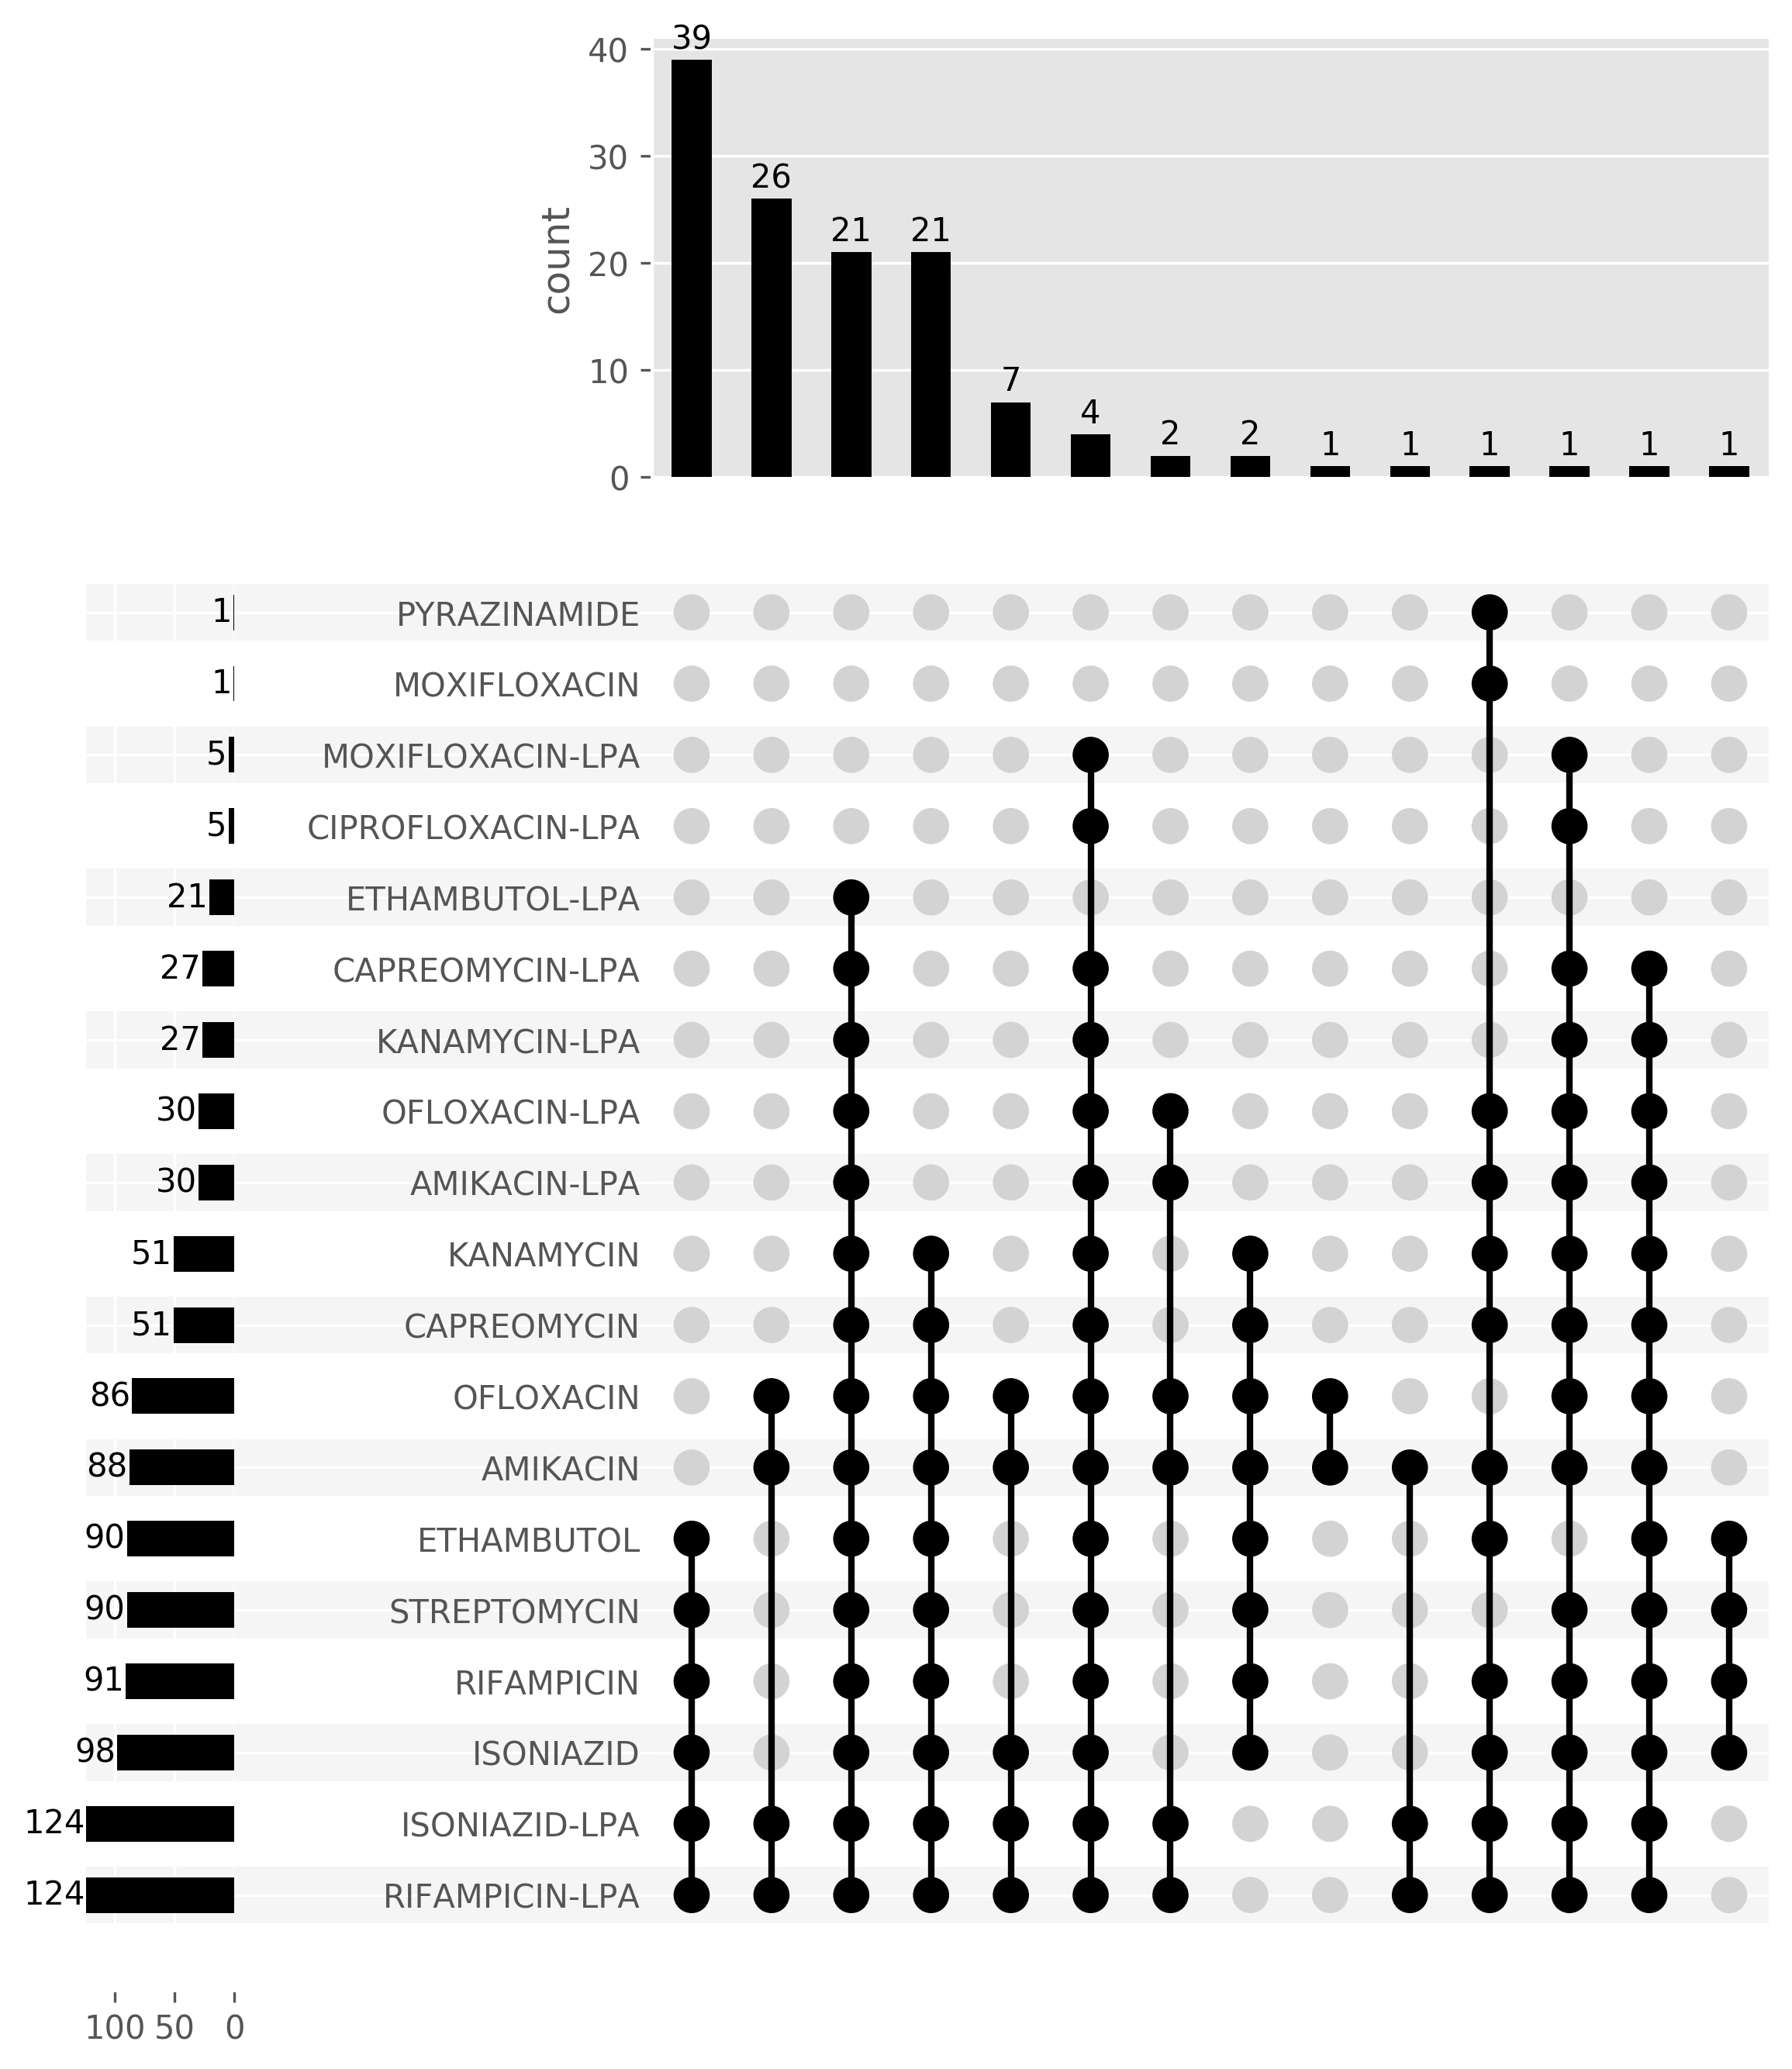
\includegraphics[width=0.90\columnwidth]{Appendix2/Figs/full-available-dst.png}
\caption{{Culture-based and line probe assay (LPA) drug susceptibility data available for samples. Each row is a drug, and the columns represent a set of samples that have phenotype information for those drugs with a filled cell. The top panel shows the number of samples in the set for that combination of drugs. The bar plot in the left panel shows the number of samples with phenotype information for that drug.
{\label{fig:full-dst}}
}}
\end{center}
\end{figure}

% ============================
\section{Constructing a panel reference graph}

\subsection{Example panel and associated VCF produced by \drprg{}}

\begin{sidewaysfigure}
\begin{Verbatim}[frame=single,framerule=0.5mm,label=Panel,fontsize=\footnotesize]
rrs     C492X   DNA     NONE
inhA    S94A    PROT    Isoniazid
\end{Verbatim}
\begin{Verbatim}[frame=single,framerule=0.5mm,label=VCF,fontsize=\footnotesize]
##INFO=<ID=RES,Number=1,Type=String,Description="Residue the variant describes (i.e. Nucleic/Amino)">
##INFO=<ID=DRUGS,Number=.,Type=String,Description="Drugs this variant causes resistance to">
##INFO=<ID=PAD,Number=1,Type=Integer,Description="Number of bases added to start and end of gene">
##INFO=<ID=ST,Number=1,Type=String,Description="Strand the gene is on">
#CHROM  POS  ID         REF  ALT     ...         INFO
rrs     592  rrs_C492X  C    A,G,T           ... PAD=100;RES=DNA;DRUGS=NONE;ST=+
inhA    380  inhA_S94A  TCG  GCT,GCC,GCA,GCG ... PAD=100;RES=PROT;DRUGS=Isoniazid;ST=+
\end{Verbatim}
\caption{An example panel (top) required by \drprg{}. The columns indicate the gene, mutation, residue the variant describes, and drug(s) the entry impacts. The panel is turned into a VCF (bottom) with proteins converted to DNA. Associated information from the panel and annotation are encoded in the \vrb{INFO} field for each entry. Note: some unnecessary information for this example is removed from the VCF entry shown here to reduce the size.}
\label{fig:example-panel}
\end{sidewaysfigure}

\subsection{Panel-based \prg{} density and haplotype problems}
\label{app:panel-prg-issues}

In the initial development stage of \drprg{}, we tried using a \prg{} built from a panel of known resistance-causing mutations (\autoref{sec:drprg-index}). However, when we began assessing the performance of \drprg{}, we discovered two common issues with this panel-based \prg{}. First, sites in certain genes were far too dense and led to many alleles having shared minimizers, thus causing shared read depth (example below). Second, the lack of haplotype information - particularly close panel variants - leads to the bulk of the missed resistance (false negative) calls. We will use two real examples to illustrate these issues.

\subsubsection{Complex \prg{} sites}
The first issue of the panel-based \prg{} mentioned above is sites in some genes being too dense (a large number of alternate alleles). This density occurs at gene locations where there are many panel variants next to each other or variants where a change to \emph{any} amino acid (denoted by \vrb{X}) leads to drug resistance. 

The reason for adjacent variants causing increased density is a parameter in \makeprg{} called the minimum match length ($m$; also discussed in \autoref{sec:improve-prg}). $m$ controls the number of base pairs that must agree between all sequences at the same position for those positions to be collapsed. Otherwise, if there is a disagreement, the alleles are split into alternate paths. 

\autoref{fig:min-match-len-example} shows an example of how $m$ can impact the structure of a \prg{}. In this example, there are three sequences with three disagreeing sites (positions 5, 9 and 13; lower-case letters; top panel). When $m=3$, there are three "neat" single-base sites, and all \vrb{A}s and \vrb{T}s are collapsed because at least three continuous bases agree between the three sequences (middle panel). However, when $m$ is increased to 4 (bottom panel), the runs of three \vrb{A}s in between the disagreeing positions are no longer collapsed. In this example, it may appear that $m=3$ has \emph{more} density, as there are more sites in total, but $m=4$ has more alternate alleles; the more there are, the greater the likelihood of them sharing minimizer \kmer{}s. 

Let us use an example of a minimizer \kmer{} of \vrb{TTTAAA} starting at position 1. When $m=4$, the top two paths (alleles) share this minimizer. As a result, if a sequencing read has that \kmer{}, both alleles have their read coverage incremented by one. However, the sequence cannot have come from two alleles.

\begin{figure}
\begin{Verbatim}[frame=single,framerule=0.5mm,label=Sequences,fontsize=\small,framesep=5mm]
TTTT*AAAgAAAgTTTT
TTTT*AAAcAAAcTTTT
TTTTtAAAtAAAtTTTT
\end{Verbatim}

\begin{Verbatim}[frame=single,framerule=0.5mm,label={$m=3$},fontsize=\small,framesep=5mm]
     *     g     g
    / \   / \   / \
TTTT   AAA-c-AAA-c-TTTT
    \ /   \ /   \ /
     t     t     t
\end{Verbatim}

\begin{Verbatim}[frame=single,framerule=0.5mm,label={$m=4$},fontsize=\small,framesep=5mm]
     *AAAgAAAg
    /         \
TTTT-*AAAcAAAc-TTTT
    \         /
     tAAAtAAAt
\end{Verbatim}
\caption{An example of how the \makeprg{} minimum match length ($m$) parameter effects \prg{} structure. The \prg{}s for three sequences (top) with three positions of difference (lower-case letters) are shown. $m$ controls when sequence is collapsed. When $m=3$ (middle), all runs of \vrb{A} and \vrb{T} are collapsed because at least three continuous bases agree between the three sequences. However, when $m=4$ (bottom), the \vrb{A}s are no longer collapsed, leaving a single, longer branched path for each sequence, rather than the three smaller, single-base paths when $m=3$. \vrb{*} is a placeholder to indicate an insertion/deletion.}
\label{fig:min-match-len-example}
\end{figure}

The issue of shared minimizer \kmer{}s in dense regions of the panel-based \prg{} led to many \drprg{} prediction errors (\drprg{} uses \pandora{} to facilitate this - \autoref{sec:drprg-predict}). One such example from real data is shown in \autoref{fig:example-pncA-dense}, which focuses on the \textit{pncA} mutation S65F. In this example, the panel-based \prg{} (top panel) has 126 alternate alleles due to many variants within less than $m$ positions of each other. In the alleles shown, there is a lot of shared sequence, and as a result, when looking at the coverage information (\vrb{MEAN\_FWD\_COVG} and \vrb{MEAN\_REV\_COVG}), we can see that \emph{all} alleles have what looks to be confident read depth. However, biologically, we know that it is \emph{extremely} unlikely there are 126 different strains in this sample; the null genotype call and low genotype confidence also corroborate this. Because no genotype can be confidently called, the prediction for this sample is susceptible (\vrb{PREDICT} tag in the VCF entry).

In contrast, when using the population-based \prg{} (bottom panel), we see a very different variant record. First, there are now only two alternate alleles indicating that in the population, there is not as much variation at this site as the panel-based \prg{} would suggest. Second, due to this reduced density, the coverage information is much "cleaner", and the genotyping much more confident. Subsequently, we now (correctly) classify this sample as having the S65F mutation in \textit{pncA}, leading to a resistance prediction.

The scenario in \autoref{fig:example-pncA-dense} was repeatedly encountered across the samples in this study. It was particularly common in genes with a lot of mutations in close proximity, such as \textit{pncA}, \textit{katG}, and \textit{rpoB}. Switching to the use of a population-based \prg{} helped reduce the majority of density-related errors that were being made by \drprg{}.

\begin{figure}
\begin{Verbatim}[breaklines=true,breakanywhere=true,frame=single,framerule=0.5mm,fontsize=\footnotesize,label=\textit{pncA} mutation S65F VCF entry for panel-based \prg{}]
#CHROM  POS     ID      REF     ALT     QUAL    FILTER  INFO    FORMAT  sample
pncA    284     5bf4ae25        CCGGACTATTCCTCGTCGTGGCCACCGCATTGC       AGAGACTATTCCTCGTCGTGGCCACCGCATTGC,AGCGACTATTCCTCGTCGTGGCCACCGCATTGC,AGGGACTATTCCTCGTCGTGGCCACCGCATTGC,AGTGACTATTCCTCGTCGTGGCCACCGCATTGC,CAAGACTATTCCTCGTCGTGGCCACCGCATTGC,CAGGACTATTCCTCGTCGTGGCCACCGCATTGC,CCAGACTATTCCTCGTCGTGGCCACCGCATTGC,CCCGACTATTCCTCGTCGTGGCCACCGCATTGC,CCGCACTATTCCTCGTCGTGGCCACCGCATTGC,CCGCATTATTCCTCGTCGTGGCCACCGCATTGC,CCGGAATATTCCTCGTCGTGGCCACCGCATTGC,CCGGACTAATCCTCGTCGTGGCCACCGCATTGC,CCGGACTAGTCCTCGTCGTGGCCACCGCATTGC,CCGGACTATTCCCCATCGTGGCCACCGCATTGC,CCGGACTATTCCCCCTCGTGGCCACCGCATTGC,CCGGACTATTCCCCGTCGTGGCCACCGCATTGC,<110 hidden>  .       frs      VARID=pncA_S65F,<rest hidden>;PREDICT=S,<rest hidden>       GT:MEAN_FWD_COVG:MEAN_REV_COVG:GT_CONF      .:31,14,14,12,14,12,13,20,20,17,17,22,20,16,20,20,<110 hidden>:29,14,16,13,15,13,13,20,21,17,17,21,20,16,20,20,<110 hidden>:14.4118
\end{Verbatim}
\begin{Verbatim}[breaklines=true,breakanywhere=true,frame=single,framerule=0.5mm,fontsize=\footnotesize,label=\textit{pncA} mutation S65F VCF entry for population-based \prg{}]
#CHROM  POS     ID      REF     ALT     QUAL    FILTER  INFO    FORMAT  sample
pncA    292     f2ff5236        TTCC    TATCT,TTTC      .       PASS    VARID=pncA_S65F,<rest hidden>;PREDICT=R,<rest hidden>   GT:MEAN_FWD_COVG:MEAN_REV_COVG:GT_CONF     2:6,0,19:9,0,26:179.789
\end{Verbatim}
\caption{Contrasting examples of the same \textit{pncA} variant site (S65F) from a panel-based \prg{} (top) and a population-based \prg{} (bottom). \vrb{VARID} indicates the panel variants this site overlaps, and \vrb{PREDICT} is the resistance prediction for the relevant \vrb{VARID}. \vrb{MEAN\_FWD\_COVG} and \vrb{MEAN\_REV\_COVG} specify the mean forward and reverse \kmer{} coverage on minimizer \kmer{}s that overlap this site. Note: due to a large number of alternate alleles (126) in the panel-based record and overlapping \vrb{VARID}s, some data has been elided for illustrative purposes.}
\label{fig:example-pncA-dense}
\end{figure}

\subsubsection{Lack of haplotype information}

The second panel-based \prg{} problem mentioned was the lack of haplotype information. This issue is of particular relevance to close panel variants and was the cause of many missed resistance calls when using the panel-based \prg{}. Additionally, we raised it in \autoref{sec:improve-prg} as an avenue for improvement when building \prg{}s.

When constructing a panel-based \prg{}, as outlined in \autoref{sec:drprg-index}, the use of haplotype information is not possible. The variants in the panel do not have accompanying data indicating what other variants they do or do not occur in tandem with. As a result, when two variants occur within $m$ base pairs of each other, the co-occurrence of the two in the same allele is not possible. For example, in \autoref{fig:min-match-len-example}, when $m=3$, it is possible to take a path through the \prg{} which would yield a sequence containing the three variants \vrb{t}, \vrb{g}, and \vrb{c}. However, when $m=4$, such a path is not possible as all possible combinations of variants are not allowed. This failure to construct all possible combinations of haplotypes is a feature of \makeprg{} and avoids combinatorial "explosions" that would occur - e.g., in the example of $m=4$, there are 18 possible recombinants of the variants that would need to be listed.

A common site where this lack of haplotype information was causing a lot of missed resistance is shown in \autoref{fig:example-gyrA-dense}. This site occurs in the \textit{gyrA} gene and is known to cause resistance to fluoroquinolones. Of relevance to the haplotype scenario we are discussing are the mutations at codons 94 and 95. An amino acid change from aspartic acid (D) at codon 94 is known to cause resistance, while the mutation of serine (S) to threonine (T) at position 95 is a common polymorphism not related to resistance \cite{sreevatsan1997,Giannoni2005,singhal2016}. Indeed, the S95T variant is so common, it is used in a line probe assay for fluoroquinolones \cite{Giannoni2005}. S95T can co-occur with D94 mutations, but due to this haplotype issue, there are no alternate alleles with a combination of the resistance-causing mutation and the natural polymorphism (the last ALT in \autoref{fig:example-gyrA-dense} top represents S95T). The sample in \autoref{fig:example-gyrA-dense} has both the D94N and S95T mutations. This combination does not occur in the panel-based \prg{} - leading to no coverage on any alleles (top panel). However, the allele combination \emph{is} found in the population-based \prg{} (bottom panel), allowing correct genotyping and thus (correctly) calling resistance to fluoroquinolones.

One conceivable way to avoid this haplotype problem would be to reduce the value of $m$. As we see in \autoref{fig:min-match-len-example}, if $m$ is low enough, the variants can be separated by matching sequence, thus allowing recombinant paths through the \prg{}; however, there are two drawbacks to this approach. First, if two variants occur directly next to each other, even $m=1$ will be unable to separate them by matching sequence. Second, there is an inverse relationship between $m$ and indexing runtime and size; as $m$ decreases, indexing the \prg{} takes longer as there are more paths to walk, and its size increases for the same reason (i.e., more minimizer \kmer{}s).

In these situations, we would expect \denovo{} variant discovery to be able to recover the correct allele combination. However, we found it struggled to do so due to the choice of maximum likelihood (ML) path in the beginning. As mentioned in \autoref{sec:seq-inference}, after \pandora{} assigns \kmer{} coverage (hits) to the local \prg{}s, it uses dynamic programming to select the ML path through each. In the panel-based \prg{} example in \autoref{fig:example-gyrA-dense}, because there is no coverage on any allele, the ML path is effectively a random choice at this site. As such, if the random choice is quite different to the allele present in the sample, the \denovo{} variant discovery step is unable to find anchor \kmer{}s (\autoref{sec:path-enum}) and thus cannot perform local assembly on the region.

Ultimately, the easiest way to solve the lack of haplotype information was to build the \prg{} from a cross-section of variation seen in a population. As we ensure there is enough diversity in the sampled population (\autoref{sec:tbprg}), the commonly occurring allele combinations are present in the final \prg{}.

\begin{figure}
\begin{Verbatim}[breaklines=true,breakanywhere=true,frame=single,framerule=0.5mm,fontsize=\footnotesize,label=\textit{gyrA} mutation S95T VCF entry for panel-based \prg{}]
#CHROM  POS     ID      REF     ALT     QUAL    FILTER  INFO    FORMAT  sample
gyrA    380     164fc346        GACAG     AACAG,AATAG,CACAG,CATAG,GCAAG,GCCAG,GCGAG,GCTAG,GGAAG,GGCAG,GGGAG,GGTAG,TACAG,TATAG,TGCAG,TGTAG,GACAC .       ld;lgc  VARID=gyrA_D94N,gyrA_D94H,gyrA_D94A,gyrA_D94G,gyrA_D94Y,gyrA_D94C,gyrA_S95T;PREDICT=S,S,S,S,S,S,S  GT:MEAN_FWD_COVG:MEAN_REV_COVG:GT_CONF     .:0,0,0,0,0,0,0,0,0,0,0,0,0,0,0,0,0,0:0,0,0,0,0,0,0,0,0,0,0,0,0,0,0,0,0,0:0
\end{Verbatim}
\begin{Verbatim}[breaklines=true,breakanywhere=true,frame=single,framerule=0.5mm,fontsize=\footnotesize,label=\textit{gyrA} mutation S95T VCF entry for population-based \prg{}]
#CHROM  POS     ID      REF     ALT     QUAL    FILTER  INFO    FORMAT  sample
gyrA    380     01a6abfd        GACAG   AACAC,CACAC,GACAC,GCCAC,GGCAC,TACAC,TACAG       .       PASS    VARID=gyrA_D94N,gyrA_D94H,gyrA_D94A,gyrA_D94G,gyrA_D94Y,gyrA_D94C,gyrA_S95T;PREDICT=R,S,S,S,S,S,S      GT:MEAN_FWD_COVG:MEAN_REV_COVG:GT_CONF     1:0,38,0,0,13,0,0,0:0,24,0,0,25,0,0,0:117.539
\end{Verbatim}
\caption{Contrasting examples of the same \textit{gyrA} variant site from a panel-based \prg{} (top) and a population-based \prg{} (bottom). \vrb{VARID} indicates the panel variants this site overlaps and \vrb{PREDICT} is the resistance prediction for the relevant \vrb{VARID}. \vrb{MEAN\_FWD\_COVG} and \vrb{MEAN\_REV\_COVG} specify the mean forward and reverse \kmer{} coverage on minimizer \kmer{}s that overlap this site.}
\label{fig:example-gyrA-dense}
\end{figure}

% =====================
\section{Example \drprg{} prediction report}

\autoref{fig:example-drprg-report} is an example of the JSON file output from \drprg{} \vrb{predict} (see \autoref{sec:drprg-predict}). This JSON file shows the resistance prediction for each drug and the supporting evidence. It has had some drugs removed for brevity.

\begin{figure}
\begin{minted}[frame=single,framerule=0.5mm,fontsize=\footnotesize]{json}
{
  "sample": "R21770",
  "susceptibility": {
    "Amikacin": {
      "evidence": [],
      "predict": "S"
    },
    "Ethambutol": {
      "evidence": [
        {
          "gene": "embB",
          "residue": "DNA",
          "variant": "G2995A",
          "vcfid": "4a883e71"
        }
      ],
      "predict": "U"
    },
    "Isoniazid": {
      "evidence": [],
      "predict": "S"
    },
    "Ofloxacin": {
      "evidence": [],
      "predict": "S"
    },
    "Pyrazinamide": {
      "evidence": [],
      "predict": "S"
    },
    "Rifampicin": {
      "evidence": [
        {
          "gene": "rpoB",
          "residue": "PROT",
          "variant": "L430X",
          "vcfid": "52981ff5"
        }
      ],
      "predict": "R"
    },
    "Streptomycin": {
      "evidence": [],
      "predict": "S"
    }
  }
}
\end{minted}
\caption{An example drug susceptibility JSON report file produced by \drprg{}. The report maps a drug to its prediction and any relevant evidence supporting that prediction. Note, evidence for susceptibility (\vrb{"S"}) predictions is not provided as susceptibility is assumed where no \vrb{R/U} prediction is made. S=susceptible; U=unknown (i.e., novel variant); R=resistant.}
\label{fig:example-drprg-report}
\end{figure}

% =====================
\section{Adjustment of default \mykrobe{} \ont{} settings}
\label{app:mykrobe-settings}

During the process of gathering the resistance prediction results in \autoref{sec:pheno-concordance} and \autoref{sec:geno-concordance}, we investigated whether the \mykrobe{} default parameters for \ont{} are optimal. Since they were calibrated on only five samples \cite{hunt2019}. In addition, we look at the impact of changing the default Illumina expected error rate (0.05) to the reported 0.001 \cite{manley2016}.

The \ont{} preset in \mykrobe{} sets the expected error rate to 0.15, the ploidy model to haploid, and ignores calls below the 90\% confidence threshold (as judged by simulating confidence scores from those present in the data) \cite{hunt2019}. Instead, we disable this preset and change the expected error rate to 0.08, leave the ploidy as haploid (avoiding minor resistance calls), and turn off the confidence threshold simulations.

The results of these parameter changes are shown in \autoref{fig:mykrobe-settings-pheno} and summarised in \autoref{tab:mykrobe-settings-pheno} for concordance with phenotype (see \autoref{sec:pheno-concordance}). In addition, as culture-based phenotypes are not available for all drugs and samples, we compare the concordance of \ont{} predictions with Illumina in \autoref{fig:mykrobe-settings-geno} and \autoref{tab:mykrobe-settings-geno}.

When comparing the WGS concordance with culture-based phenotypes, these results reveal that the default \ont{} settings for \mykrobe{} lead to a much higher number of missed resistance (FN) classifications for all drugs when compared to the adjusted settings. However, the default settings do lead to fewer false-positive predictions for all drugs. Additionally, the adjusted Illumina error rate led to one FN being recovered (classified TP) for ethambutol and unchanged classifications for everything else.

\ont{} concordance with Illumina predictions shows default settings lead to more FN calls than with adjusted settings, especially for the first-line drugs ethambutol, isoniazid, and rifampicin. The adjusted settings for \mykrobe{} led to quite similar predictions between \ont{} and Illumina. Additionally, they lead to much less \ont{} missed resistance calls but more false positives. However, missed resistance is generally deemed a "worse" error, and as such, for the work in \autoref{chap:dst} we chose to use these adjusted parameters for \mykrobe{}.

\begin{figure}
\begin{center}
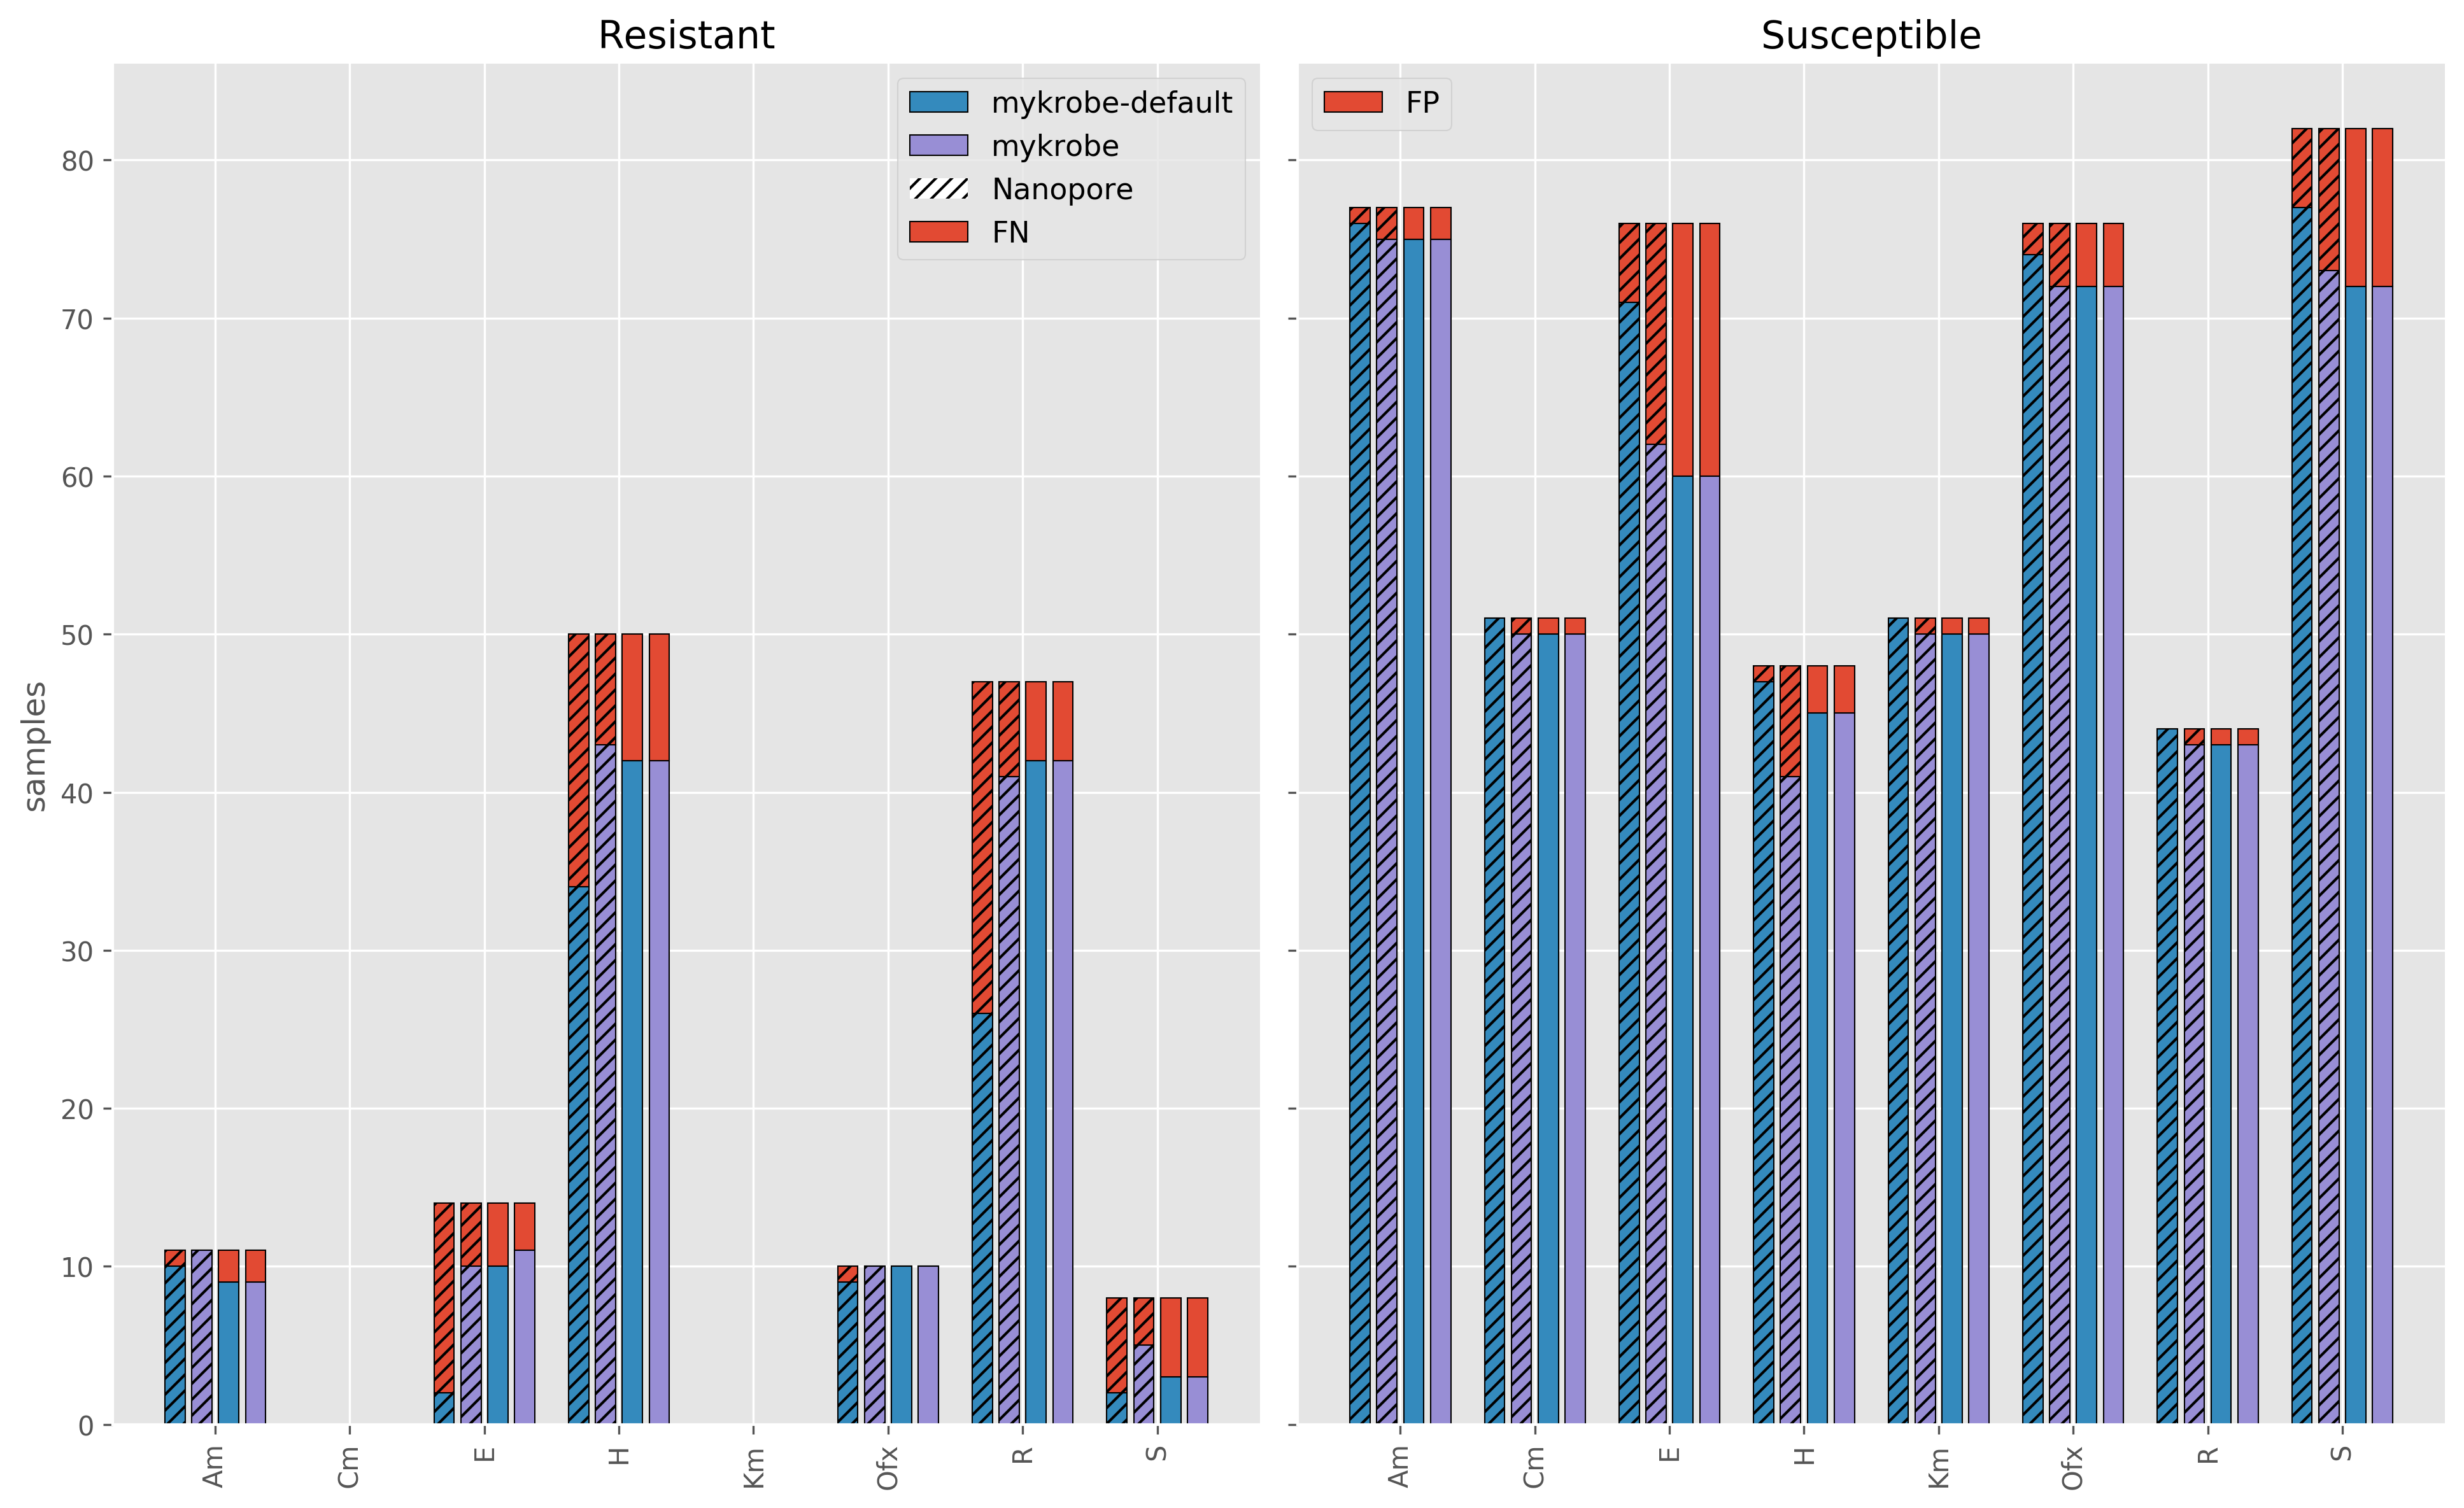
\includegraphics[width=0.90\columnwidth]{Appendix2/Figs/mykrobe_settings_pheno.png}
\caption{{Number of resistant (left) and susceptible (right) culture-based drug susceptibility phenotypes correctly identified by \mykrobe{} with default (blue) or adjusted (purple) settings. \ont{} data is indicated by diagonal stripes, with Illumina having no stripes. The red bars indicate missed (FN) or incorrect (FP) predictions. The x-axis shows the drugs with available phenotype data. E - ethambutol; H - isoniazid; R - rifampicin; S - streptomycin; Km - kanamycin; Am - amikacin; Ofx - ofloxacin; Cm - capreomycin.
{\label{fig:mykrobe-settings-pheno}}
}}
\end{center}
\end{figure}

\begin{table}
\centering
\resizebox{\textwidth}{!}{%
\begin{tabular}{@{}lllllllll@{}}
\toprule
Drug &
  Technology &
  \mykrobe{} &
  FN(R) &
  FP(S) &
  FNR(95\% CI) &
  FPR(95\% CI) &
  PPV(95\% CI) &
  NPV(95\% CI) \\ \midrule
\multirow{4}{*}{Amikacin} &
  \multirow{2}{*}{\ont{}} &
  \mykrobe{}-default &
  1(11) &
  1(77) &
  9.1\% (1.6-37.7\%) &
  1.3\% (0.2-7.0\%) &
  90.9\% (62.3-98.4\%) &
  98.7\% (93.0-99.8\%) \\
 &
   &
  \mykrobe{} &
  0(11) &
  2(77) &
  0.0\% (0.0-25.9\%) &
  2.6\% (0.7-9.0\%) &
  84.6\% (57.8-95.7\%) &
  100.0\% (95.1-100.0\%) \\
 &
  \multirow{2}{*}{Illumina} &
  \mykrobe{}-default &
  2(11) &
  2(77) &
  18.2\% (5.1-47.7\%) &
  2.6\% (0.7-9.0\%) &
  81.8\% (52.3-94.9\%) &
  97.4\% (91.0-99.3\%) \\
 &
   &
  \mykrobe{} &
  2(11) &
  2(77) &
  18.2\% (5.1-47.7\%) &
  2.6\% (0.7-9.0\%) &
  81.8\% (52.3-94.9\%) &
  97.4\% (91.0-99.3\%) \\ \\ \cmidrule(l){3-9} 
\multirow{4}{*}{Capreomycin} &
  \multirow{2}{*}{\ont{}} &
  \mykrobe{}-default &
  0(0) &
  0(51) &
  - &
  0.0\% (0.0-7.0\%) &
  - &
  100.0\% (93.0-100.0\%) \\
 &
   &
  \mykrobe{} &
  0(0) &
  1(51) &
  - &
  2.0\% (0.3-10.3\%) &
  0.0\% (0.0-79.3\%) &
  100.0\% (92.9-100.0\%) \\
 &
  \multirow{2}{*}{Illumina} &
  \mykrobe{}-default &
  0(0) &
  1(51) &
  - &
  2.0\% (0.3-10.3\%) &
  0.0\% (0.0-79.3\%) &
  100.0\% (92.9-100.0\%) \\
 &
   &
  \mykrobe{} &
  0(0) &
  1(51) &
  - &
  2.0\% (0.3-10.3\%) &
  0.0\% (0.0-79.3\%) &
  100.0\% (92.9-100.0\%) \\ \\ \cmidrule(l){3-9} 
\multirow{4}{*}{Ethambutol} &
  \multirow{2}{*}{\ont{}} &
  \mykrobe{}-default &
  12(14) &
  5(76) &
  85.7\% (60.1-96.0\%) &
  \textbf{6.6\% (2.8-14.5\%)} &
  28.6\% (8.2-64.1\%) &
  85.5\% (76.4-91.5\%) \\
 &
   &
  \mykrobe{} &
  4(14) &
  14(76) &
  \textbf{28.6\% (11.7-54.6\%)} &
  18.4\% (11.3-28.6\%) &
  41.7\% (24.5-61.2\%) &
  93.9\% (85.4-97.6\%) \\
 &
  \multirow{2}{*}{Illumina} &
  \mykrobe{}-default &
  4(14) &
  16(76) &
  28.6\% (11.7-54.6\%) &
  21.1\% (13.4-31.5\%) &
  38.5\% (22.4-57.5\%) &
  93.8\% (85.0-97.5\%) \\
 &
   &
  \mykrobe{} &
  3(14) &
  16(76) &
  21.4\% (7.6-47.6\%) &
  21.1\% (13.4-31.5\%) &
  40.7\% (24.5-59.3\%) &
  95.2\% (86.9-98.4\%) \\ \\ \cmidrule(l){3-9} 
\multirow{4}{*}{Isoniazid} &
  \multirow{2}{*}{\ont{}} &
  \mykrobe{}-default &
  16(50) &
  1(48) &
  32.0\% (20.8-45.8\%) &
  \textbf{2.1\% (0.4-10.9\%)} &
  97.1\% (85.5-99.5\%) &
  74.6\% (62.7-83.7\%) \\
 &
   &
  \mykrobe{} &
  7(50) &
  7(48) &
  \textbf{14.0\% (7.0-26.2\%)} &
  14.6\% (7.2-27.2\%) &
  86.0\% (73.8-93.0\%) &
  85.4\% (72.8-92.8\%) \\
 &
  \multirow{2}{*}{Illumina} &
  \mykrobe{}-default &
  8(50) &
  3(48) &
  16.0\% (8.3-28.5\%) &
  6.2\% (2.1-16.8\%) &
  93.3\% (82.1-97.7\%) &
  84.9\% (72.9-92.1\%) \\
 &
   &
  \mykrobe{} &
  8(50) &
  3(48) &
  16.0\% (8.3-28.5\%) &
  6.2\% (2.1-16.8\%) &
  93.3\% (82.1-97.7\%) &
  84.9\% (72.9-92.1\%) \\ \\ \cmidrule(l){3-9} 
\multirow{4}{*}{Kanamycin} &
  \multirow{2}{*}{\ont{}} &
  \mykrobe{}-default &
  0(0) &
  0(51) &
  - &
  0.0\% (0.0-7.0\%) &
  - &
  100.0\% (93.0-100.0\%) \\
 &
   &
  \mykrobe{} &
  0(0) &
  1(51) &
  - &
  2.0\% (0.3-10.3\%) &
  0.0\% (0.0-79.3\%) &
  100.0\% (92.9-100.0\%) \\
 &
  \multirow{2}{*}{Illumina} &
  \mykrobe{}-default &
  0(0) &
  1(51) &
  - &
  2.0\% (0.3-10.3\%) &
  0.0\% (0.0-79.3\%) &
  100.0\% (92.9-100.0\%) \\
 &
   &
  \mykrobe{} &
  0(0) &
  1(51) &
  - &
  2.0\% (0.3-10.3\%) &
  0.0\% (0.0-79.3\%) &
  100.0\% (92.9-100.0\%) \\ \\ \cmidrule(l){3-9} 
\multirow{4}{*}{Ofloxacin} &
  \multirow{2}{*}{\ont{}} &
  \mykrobe{}-default &
  1(10) &
  2(76) &
  10.0\% (1.8-40.4\%) &
  2.6\% (0.7-9.1\%) &
  81.8\% (52.3-94.9\%) &
  98.7\% (92.8-99.8\%) \\
 &
   &
  \mykrobe{} &
  0(10) &
  4(76) &
  0.0\% (-0.0-27.8\%) &
  5.3\% (2.1-12.8\%) &
  71.4\% (45.4-88.3\%) &
  100.0\% (94.9-100.0\%) \\
 &
  \multirow{2}{*}{Illumina} &
  \mykrobe{}-default &
  0(10) &
  4(76) &
  0.0\% (-0.0-27.8\%) &
  5.3\% (2.1-12.8\%) &
  71.4\% (45.4-88.3\%) &
  100.0\% (94.9-100.0\%) \\
 &
   &
  \mykrobe{} &
  0(10) &
  4(76) &
  0.0\% (-0.0-27.8\%) &
  5.3\% (2.1-12.8\%) &
  71.4\% (45.4-88.3\%) &
  100.0\% (94.9-100.0\%) \\ \\ \cmidrule(l){3-9} 
\multirow{4}{*}{Rifampicin} &
  \multirow{2}{*}{\ont{}} &
  \mykrobe{}-default &
  21(47) &
  0(44) &
  44.7\% (31.4-58.8\%) &
  0.0\% (0.0-8.0\%) &
  100.0\% (87.1-100.0\%) &
  67.7\% (55.6-77.8\%) \\
 &
   &
  \mykrobe{} &
  6(47) &
  1(44) &
  \textbf{12.8\% (6.0-25.2\%)} &
  2.3\% (0.4-11.8\%) &
  97.6\% (87.7-99.6\%) &
  87.8\% (75.8-94.3\%) \\
 &
  \multirow{2}{*}{Illumina} &
  \mykrobe{}-default &
  5(47) &
  1(44) &
  10.6\% (4.6-22.6\%) &
  2.3\% (0.4-11.8\%) &
  97.7\% (87.9-99.6\%) &
  89.6\% (77.8-95.5\%) \\
 &
   &
  \mykrobe{} &
  5(47) &
  1(44) &
  10.6\% (4.6-22.6\%) &
  2.3\% (0.4-11.8\%) &
  97.7\% (87.9-99.6\%) &
  89.6\% (77.8-95.5\%) \\ \\ \cmidrule(l){3-9} 
\multirow{4}{*}{Streptomycin} &
  \multirow{2}{*}{\ont{}} &
  \mykrobe{}-default &
  6(8) &
  5(82) &
  75.0\% (40.9-92.9\%) &
  \textbf{6.1\% (2.6-13.5\%)} &
  28.6\% (8.2-64.1\%) &
  92.8\% (85.1-96.6\%) \\
 &
   &
  \mykrobe{} &
  3(8) &
  9(82) &
  \textbf{37.5\% (13.7-69.4\%)} &
  11.0\% (5.9-19.6\%) &
  35.7\% (16.3-61.2\%) &
  96.1\% (89.0-98.6\%) \\
 &
  \multirow{2}{*}{Illumina} &
  \mykrobe{}-default &
  5(8) &
  10(82) &
  62.5\% (30.6-86.3\%) &
  12.2\% (6.8-21.0\%) &
  23.1\% (8.2-50.3\%) &
  93.5\% (85.7-97.2\%) \\
 &
   &
  \mykrobe{} &
  5(8) &
  10(82) &
  62.5\% (30.6-86.3\%) &
  12.2\% (6.8-21.0\%) &
  23.1\% (8.2-50.3\%) &
  93.5\% (85.7-97.2\%) \\ \cmidrule(l){3-9} 
\end{tabular}%
}
\caption{Comparison of WGS drug resistance predictions with culture-based phenotype. For this comparison, we assume the culture-based phenotype is correct and evaluate \mykrobe{} with default and adjusted settings for Illumina and \ont{} resistance predictions accordingly. Pyrazinamide and Moxifloxacin are excluded as phenotype information is only available for one sample. Bold text is used to highlight differences of note. FN=false negative; R=number of resistant samples; FP=false positive; S=number of susceptible samples; FNR=false negative rate; FPR=false positive rate; PPV=positive predictive value; NPV=negative predictive value; CI=Wilson score confidence interval}
\label{tab:mykrobe-settings-pheno}
\end{table}

\begin{figure}
\begin{center}
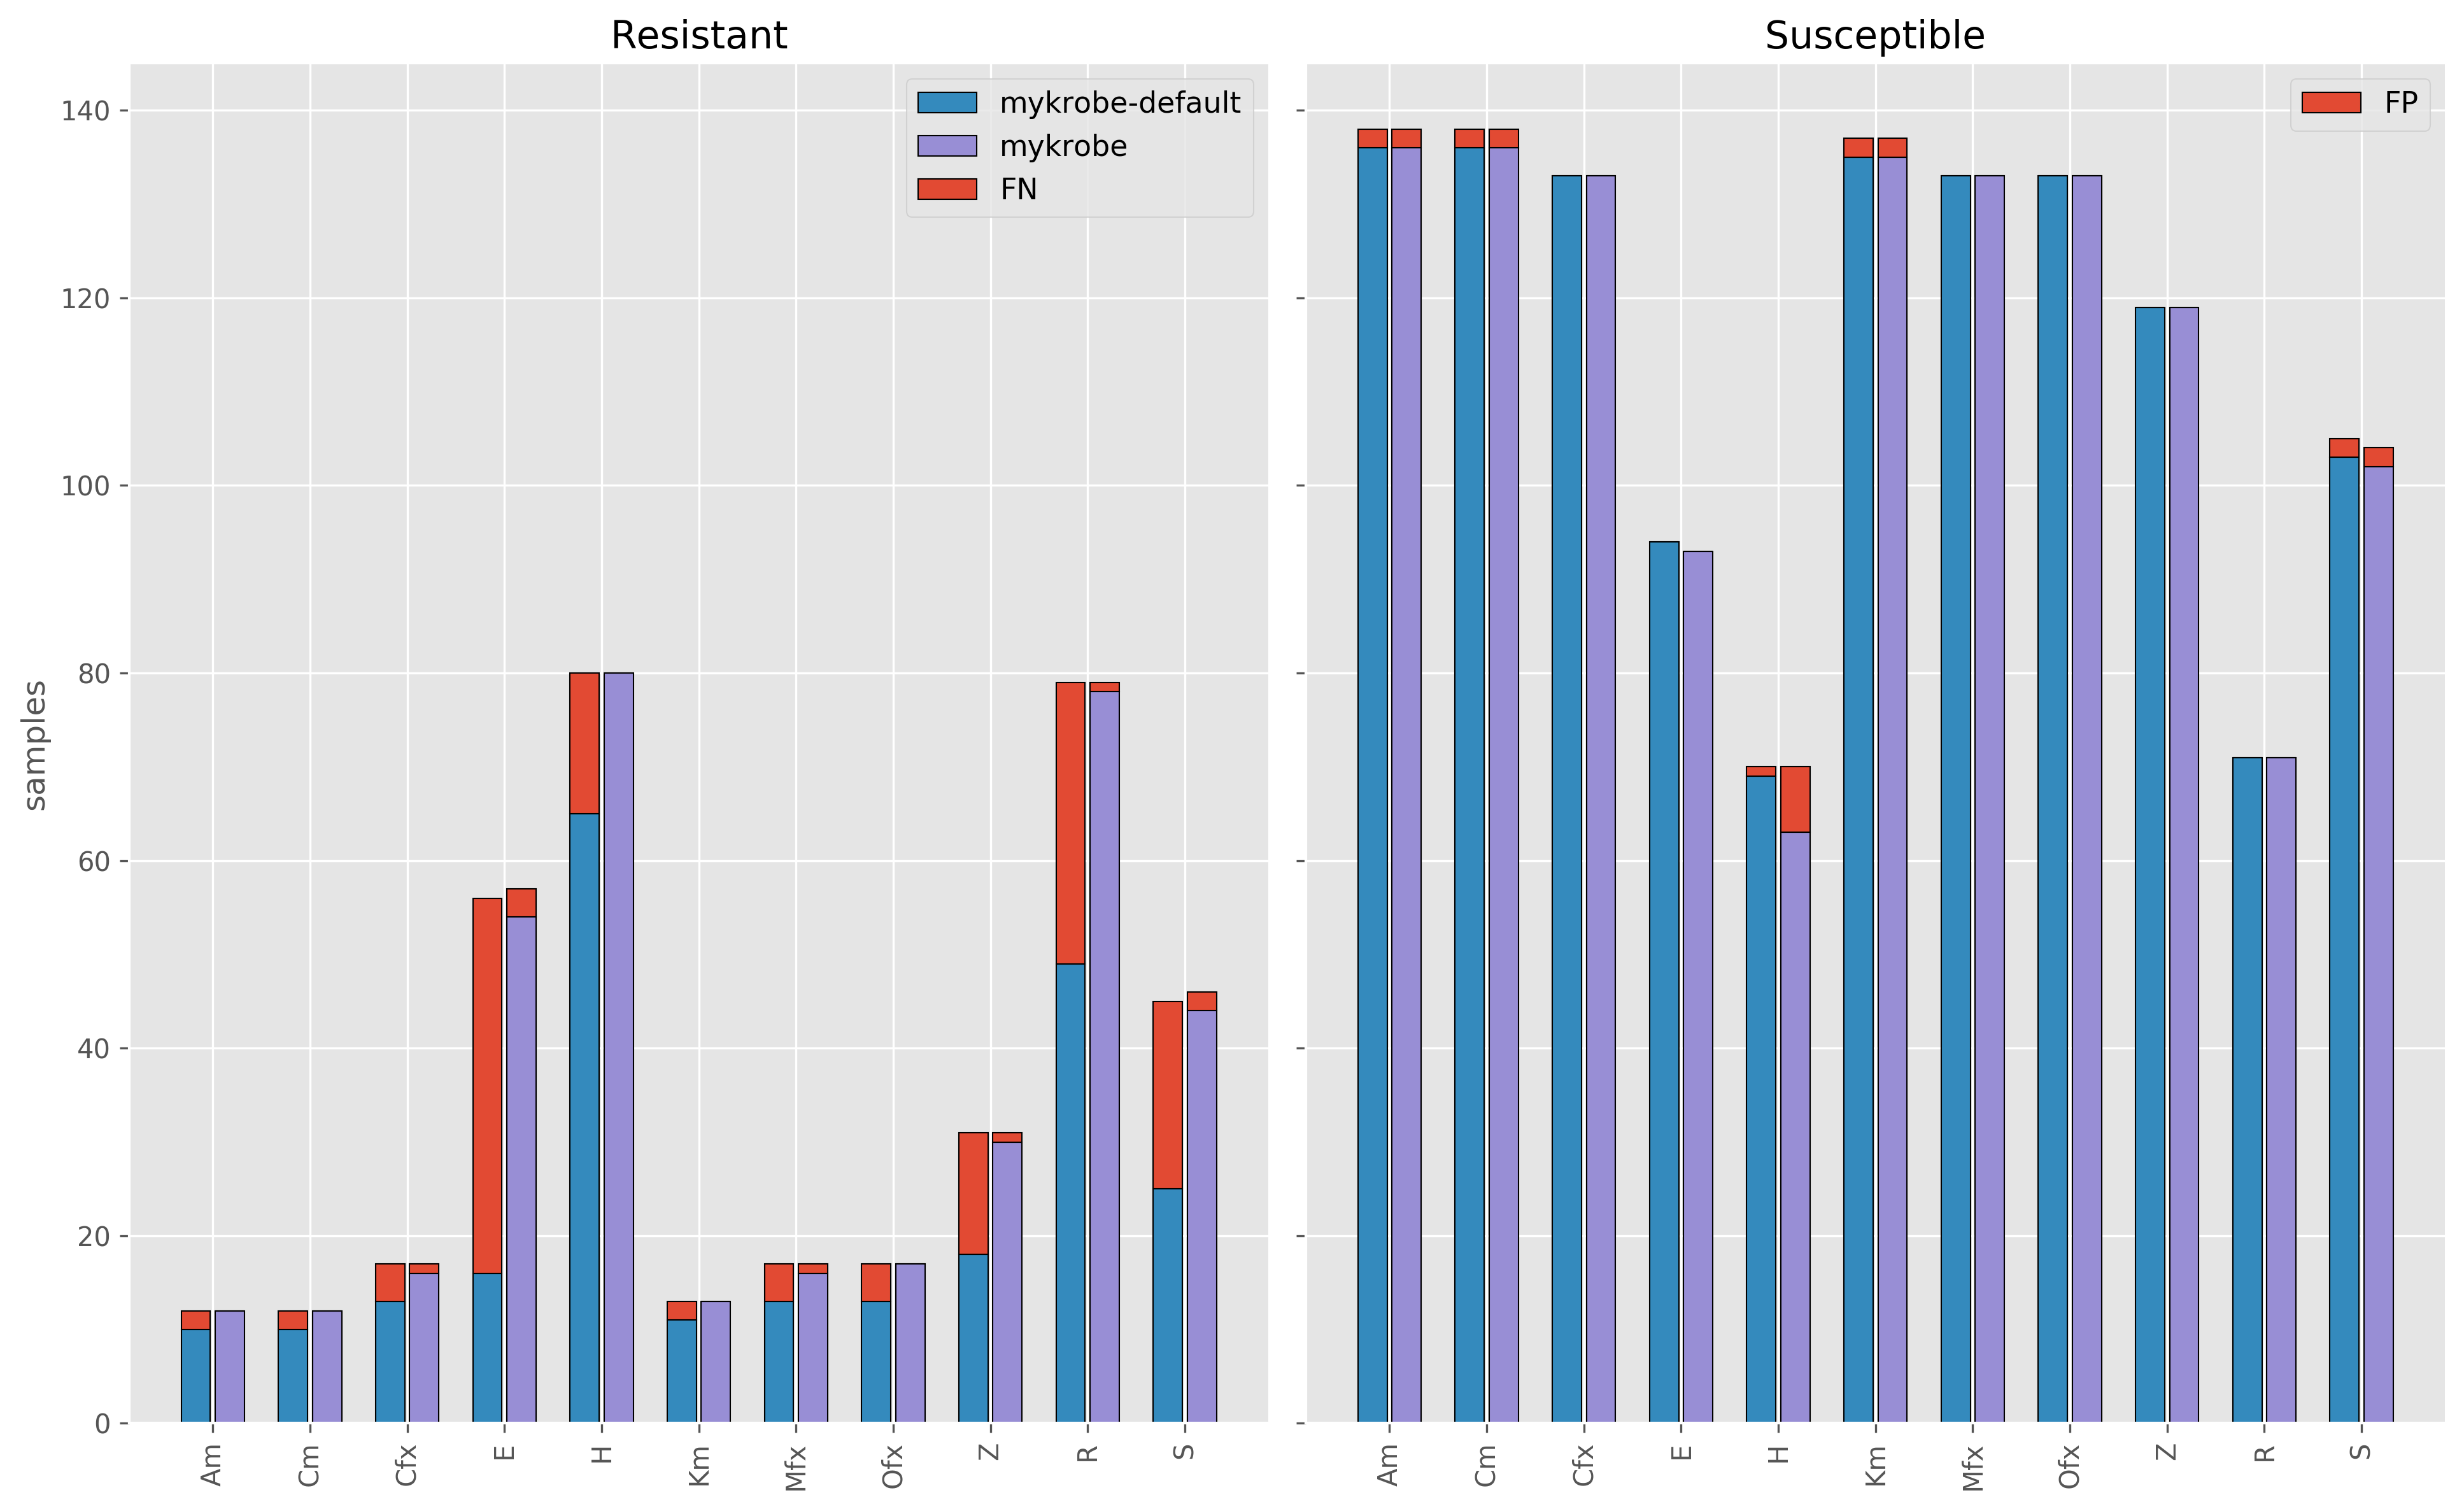
\includegraphics[width=0.90\columnwidth]{Appendix2/Figs/mykrobe_settings_illumina_concordance.png}
\caption{{Number of resistant (left) and susceptible (right) Illumina WGS-based drug susceptibility phenotypes correctly identified using \ont{} data. \ont{} predictions for \mykrobe{} with default (blue) and adjusted (purple) settings are compared to those from Illumina with the same settings. The red bars indicate missed (FN) or incorrect (FP) predictions. The x-axis shows the drugs with available phenotype data. E - ethambutol; H - isoniazid; Z - pyrazinamide; R - rifampicin; S - streptomycin; Km - kanamycin; Am - amikacin; Ofx - ofloxacin; Cm - capreomycin; Mfx - moxifloxacin.
{\label{fig:mykrobe-settings-geno}}
}}
\end{center}
\end{figure}


\begin{table}
\centering
\resizebox{\textwidth}{!}{%
\begin{tabular}{@{}llllllll@{}}
\toprule
Drug                          & Tool               & FN(R)  & FP(S)  & FNR(95\% CI)                & FPR(95\% CI)        & PPV(95\% CI)           & NPV(95\% CI)           \\ \midrule
\multirow{2}{*}{Amikacin}     & \mykrobe{}-default & 2(12)  & 2(138) & 16.7\% (4.7-44.8\%)         & 1.4\% (0.4-5.1\%)   & 83.3\% (55.2-95.3\%)   & 98.6\% (94.9-99.6\%)   \\
                              & \mykrobe{}         & 0(12)  & 2(138) & \textbf{0.0\% (0.0-24.2\%)} & 1.4\% (0.4-5.1\%)   & 85.7\% (60.1-96.0\%)   & 100.0\% (97.3-100.0\%) \\ \cmidrule(l){2-8} 
\multirow{2}{*}{Capreomycin}  & \mykrobe{}-default & 2(12)  & 2(138) & 16.7\% (4.7-44.8\%)         & 1.4\% (0.4-5.1\%)   & 83.3\% (55.2-95.3\%)   & 98.6\% (94.9-99.6\%)   \\
                              & \mykrobe{}         & 0(12)  & 2(138) & \textbf{0.0\% (0.0-24.2\%)} & 1.4\% (0.4-5.1\%)   & 85.7\% (60.1-96.0\%)   & 100.0\% (97.3-100.0\%) \\ \cmidrule(l){2-8} 
\multirow{2}{*}{Ciprofloxacin} & \mykrobe{}-default & 4(17)  & 0(133) & 23.5\% (9.6-47.3\%)  & 0.0\% (0.0-2.8\%)          & 100.0\% (77.2-100.0\%) & 97.1\% (92.7-98.9\%) \\
                              & \mykrobe{}         & 1(17)  & 0(133) & \textbf{5.9\% (1.0-27.0\%)} & 0.0\% (0.0-2.8\%)   & 100.0\% (80.6-100.0\%) & 99.3\% (95.9-99.9\%)   \\ \cmidrule(l){2-8} 
\multirow{2}{*}{Ethambutol}   & \mykrobe{}-default & 40(56) & 0(94)  & 71.4\% (58.5-81.6\%)        & 0.0\% (0.0-3.9\%)   & 100.0\% (80.6-100.0\%) & 70.1\% (61.9-77.2\%)   \\
                              & \mykrobe{}         & 3(57)  & 0(93)  & \textbf{5.3\% (1.8-14.4\%)} & 0.0\% (0.0-4.0\%)   & 100.0\% (93.4-100.0\%) & 96.9\% (91.2-98.9\%)   \\ \cmidrule(l){2-8} 
\multirow{2}{*}{Isoniazid}     & \mykrobe{}-default & 15(80) & 1(70)  & 18.8\% (11.7-28.7\%) & \textbf{1.4\% (0.3-7.7\%)} & 98.5\% (91.9-99.7\%)   & 82.1\% (72.6-88.9\%) \\
                              & \mykrobe{}         & 0(80)  & 7(70)  & \textbf{0.0\% (0.0-4.6\%)}  & 10.0\% (4.9-19.2\%) & 92.0\% (84.3-96.0\%)   & 100.0\% (94.3-100.0\%) \\ \cmidrule(l){2-8} 
\multirow{2}{*}{Kanamycin}    & \mykrobe{}-default & 2(13)  & 2(137) & 15.4\% (4.3-42.2\%)         & 1.5\% (0.4-5.2\%)   & 84.6\% (57.8-95.7\%)   & 98.5\% (94.8-99.6\%)   \\
                              & \mykrobe{}         & 0(13)  & 2(137) & \textbf{0.0\% (0.0-22.8\%)} & 1.5\% (0.4-5.2\%)   & 86.7\% (62.1-96.3\%)   & 100.0\% (97.2-100.0\%) \\ \cmidrule(l){2-8} 
\multirow{2}{*}{Moxifloxacin} & \mykrobe{}-default & 4(17)  & 0(133) & 23.5\% (9.6-47.3\%)         & 0.0\% (0.0-2.8\%)   & 100.0\% (77.2-100.0\%) & 97.1\% (92.7-98.9\%)   \\
                              & \mykrobe{}         & 1(17)  & 0(133) & \textbf{5.9\% (1.0-27.0\%)} & 0.0\% (0.0-2.8\%)   & 100.0\% (80.6-100.0\%) & 99.3\% (95.9-99.9\%)   \\ \cmidrule(l){2-8} 
\multirow{2}{*}{Ofloxacin}    & \mykrobe{}-default & 4(17)  & 0(133) & 23.5\% (9.6-47.3\%)         & 0.0\% (0.0-2.8\%)   & 100.0\% (77.2-100.0\%) & 97.1\% (92.7-98.9\%)   \\
                              & \mykrobe{}         & 0(17)  & 0(133) & \textbf{0.0\% (0.0-18.4\%)} & 0.0\% (0.0-2.8\%)   & 100.0\% (81.6-100.0\%) & 100.0\% (97.2-100.0\%) \\ \cmidrule(l){2-8} 
\multirow{2}{*}{Pyrazinamide}  & \mykrobe{}-default & 13(31) & 0(119) & 41.9\% (26.4-59.2\%) & 0.0\% (0.0-3.1\%)          & 100.0\% (82.4-100.0\%) & 90.2\% (83.9-94.2\%) \\
                              & \mykrobe{}         & 1(31)  & 0(119) & \textbf{3.2\% (0.6-16.2\%)} & 0.0\% (0.0-3.1\%)   & 100.0\% (88.6-100.0\%) & 99.2\% (95.4-99.9\%)   \\ \cmidrule(l){2-8} 
\multirow{2}{*}{Rifampicin}   & \mykrobe{}-default & 30(79) & 0(71)  & 38.0\% (28.1-49.0\%)        & 0.0\% (0.0-5.1\%)   & 100.0\% (92.7-100.0\%) & 70.3\% (60.8-78.3\%)   \\
                              & \mykrobe{}         & 1(79)  & 0(71)  & \textbf{1.3\% (0.2-6.8\%)}  & 0.0\% (0.0-5.1\%)   & 100.0\% (95.3-100.0\%) & 98.6\% (92.5-99.8\%)   \\ \cmidrule(l){2-8} 
\multirow{2}{*}{Streptomycin} & \mykrobe{}-default & 20(45) & 2(105) & 44.4\% (30.9-58.8\%)        & 1.9\% (0.5-6.7\%)   & 92.6\% (76.6-97.9\%)   & 83.7\% (76.2-89.2\%)   \\
                              & \mykrobe{}         & 2(46)  & 2(104) & \textbf{4.3\% (1.2-14.5\%)} & 1.9\% (0.5-6.7\%)   & 95.7\% (85.5-98.8\%)   & 98.1\% (93.3-99.5\%)   \\ \cmidrule(l){2-8} 
\end{tabular}%
}
\caption{Comparison of \ont{} drug resistance predictions concordance with Illumina predictions. For this comparison, we assume the \mykrobe{} resistance prediction from Illumina data is correct and evaluate the \ont{} prediction accordingly. \mykrobe{}-default and \mykrobe{} indicates \mykrobe{} with default or adjusted settings, respectively. Bold text is used to highlight differences of note. FN=false negative; R=number of resistant samples; FP=false positive; S=number of susceptible samples; FNR=false negative rate; FPR=false positive rate; PPV=positive predictive value; NPV=negative predictive value; CI=Wilson score confidence interval}
\label{tab:mykrobe-settings-geno}
\end{table}
